\documentclass[twocolumn,numberedappendix]{../aastex6}

% these lines seem necessary for pdflatex to get the paper size right
\pdfpagewidth 8.5in
\pdfpageheight 11.0in

% for the red MarginPars
\usepackage{color}

% some extra math symbols
\usepackage{mathtools}

% allows Greek symbols to be bold
\usepackage{bm}

% allows us to force the location of a figure
\usepackage{float}

% allows comment sections
\usepackage{verbatim}

% Override choices in \autoref
\def\sectionautorefname{Section}
\def\subsectionautorefname{Section}
\def\subsubsectionautorefname{Section}

% MarginPars
\setlength{\marginparwidth}{0.75in}
\newcommand{\MarginPar}[1]{\marginpar{\vskip-\baselineskip\raggedright\tiny\sffamily\hrule\smallskip{\color{red}#1}\par\smallskip\hrule}}

\newcommand{\msolar}{\mathrm{M}_\odot}

% Software names
\newcommand{\boxlib}{\texttt{BoxLib}}
\newcommand{\castro}{\texttt{CASTRO}}
\newcommand{\microphysics}{\texttt{Microphysics}}
\newcommand{\wdmerger}{\texttt{wdmerger}}
\newcommand{\python}{\texttt{Python}}
\newcommand{\matplotlib}{\texttt{matplotlib}}
\newcommand{\yt}{\texttt{yt}}
\newcommand{\vode}{\texttt{VODE}}
\newcommand{\isoseven}{\texttt{iso7}}
\newcommand{\aproxthirteen}{\texttt{aprox13}}
\newcommand{\aproxnineteen}{\texttt{aprox19}}
\newcommand{\aproxtwentyone}{\texttt{aprox21}}

\begin{document}

%==========================================================================
% Title
%==========================================================================
\title{White Dwarf Mergers on Adaptive Meshes\\ II. Collisions}

\shorttitle{WD Mergers. II. Collisions}
\shortauthors{Katz et al. (2016)}

\author{Max P. Katz\altaffilmark{1}}
\author{Michael Zingale\altaffilmark{1}}
\author{Alan C. Calder\altaffilmark{1,2}}
\author{F. Douglas Swesty\altaffilmark{1}}
\author{Ann S. Almgren\altaffilmark{3}}
\author{Weiqun Zhang\altaffilmark{3}}
\author{Frank X. Timmes\altaffilmark{4,5}}

\altaffiltext{1}
{
  Department of Physics and Astronomy,
  Stony Brook University, Stony Brook, NY, 11794-3800, USA
}

\altaffiltext{2}
{
  Institute for Advanced Computational Sciences,
  Stony Brook University, Stony Brook, NY, 11794-5250, USA
}

\altaffiltext{3}
{
  Center for Computational Sciences and Engineering,
  Lawrence Berkeley National Laboratory, Berkeley, CA 94720
}

\altaffiltext{4}
{
  The Joint Institute for Nuclear Astrophysics, USA
}

\altaffiltext{5}
{
  School of Earth and Space Exploration, Arizona State University, Tempe, AZ, USA
}



%==========================================================================
% Abstract
%==========================================================================
\begin{abstract}
Collisions of white dwarfs are a subset of white dwarf mergers that occur
when the stars approach each other nearly head-on. These have the potential
for explosive nucleosynthesis, leading to a thermonuclear detonation that
disrupts both stars, possibly causing a Type Ia supernova. Simulation of
these events is challenging due to the rapid evolution of the nuclear burning,
posing numerical challenges related to both spatial and temporal resolution.
In this study we explore a number of the algorithms that affect the outcome
of reacting hydrodynamics simulations that lead to explosive burning and
address the question of what needs to be done to ensure that these simulations
are properly converged. We find that achieving a converged simulation in the
code \castro\ is non-trivial and requires demanding computational resources.
We also discuss the quantities obtained from our simulations that bear relevance
to observations of these events, particularly production of nickel-group
elements and gravitational wave emission during the collision.
\end{abstract}
\keywords{supernovae: general - white dwarfs}

%==========================================================================
% Introduction
%==========================================================================
\section{Introduction}
\label{sec:introduction}

Binary white dwarf (WD) systems have long been thought to be potential progenitors
of Type Ia supernovae (SNe Ia) \citep{ibentutukov:1984,webbink:1984}. Recently there
has been a growing amount of observational evidence that double WD systems play
an important role in explaining at least some SNe Ia \citep{maoz:2014}. These systems
may be isolated or they may be in hierarchical triple systems, where a WD binary
system in a tight inner orbit is gravitationally coupled to a third, outer star.
In either case the binary WD pair can merge due to the emissions of gravitational waves,
but in the hierarchical triple case, dynamical interactions between the WD binary and
the outer star can prompt mergers as well \citep{thompson:2011,hamers:2013}. The mergers
occur due to perturbations in the eccentricity of the binary orbit caused by the outer
star, which significantly increase the gravitational wave emission of the system. In a
subset of these mergers the eccentricity may be driven to such a high value that the
merger resembles a head-on collision of the binary WDs. Whether the rate of these collisions
may be high enough to significantly contribute to the observed SN Ia rate is uncertain,
though \cite{katzdong:2012} suggest that this is plausible.

Over the past few years a number of groups have performed simulations of WD collisions
to understand whether they may yield astrophysical transients that look like SNe Ia
\citep{rosswog:2009,raskin:2010,loren-aguilar:2010,hawley:2012,garcia-senz:2013,
kushnir:2013,papish:2015,holcomb:2015}. Head-on collisions rapidly convert a significant
amount of kinetic energy into thermal energy in a small region and thus set up the
conditions for a thermonuclear detonation, and these previous simulations have indeed
found that detonations occur and convert a large amount of carbon/oxygen material into
iron-group elements. These papers varied significantly in the hydrodynamic methods used
(Lagrangian versus Eulerian methods), the methodology used for coupling nuclear
reactions to the hydrodynamics (including variation in the number of isotopes in
the nuclear network and in the evolution of the temperature), and the temporal and
spatial resolution. Consequently they yielded estimates of production of nickel-group
elements that varied significantly, leaving much uncertainty about how such an event
would appear observationally and whether it bears any resemblance to a SN Ia.
See Table 4 of \cite{garcia-senz:2013} for a summary of the outcome of many of these studies.

In this paper we seek to add another view to the problem using the reactive hydrodynamics
code \castro\ \citep{castro} and its underlying adaptive mesh refinement library \boxlib.
This paper is a follow-up to \citet{wdmergerI} (hereafter, Paper I), which established
the hydrodynamic methdology we are using to simulate mergers of white dwarfs.
Paper I left out a discussion of the methodology we are using for nuclear reactions,
and we fill out this information below in \autoref{sec:numericalmethods}. While it is
our aim is to add information to the discussion about collisions of white dwarfs,
we also view this work as a methodology study that asks to what extent we
can trust the reliability of explosive thermonuclear reactions in Eulerian
hydrodynamics simulations. As a corollary, to what extent does static and/or
adaptive mesh refinement resolve the types of problems that occur in low resolution
simulations? We discuss this in Section \autoref{sec:resolution}, though first
we examine the response of the code to a number of user-specified parameters in
\autoref{sec:parameters}. We then close with our thoughts on what our work implies
for the broader astrophysical reacting hydrodynamics literature in \autoref{sec:conclusion}.



%==========================================================================
% Numerical Implementation
%==========================================================================
\section{Numerical Methods}
\label{sec:numericalmethods}

The hydrodynamical equations solved in this paper were presented in \citet{wdmergerI} (hereafter, Paper I).
In this paper we focus our discussion on our implementation of the nuclear
reaction network and integrator. There are three main areas of concern: first,
specifying what nuclides are in the network and what reaction rates link the
various nuclides; second, once the system of ODEs governing the evolution of
the nuclear species has been written down, how to couple them to ODEs governing
the evolution of the thermodynamics, in particular the temperature; third,
coupling the nuclear reaction updates to the evolution of the hydrodynamical
system. We will deal with each of these in turn in the following subsections.

\subsection{Nuclear Network}
\label{sec:network}

White dwarfs are mainly composed of $\alpha$-chain particles, primarily ${}^4$He,
${}^{12}$C, ${}^{16}$O, ${}^{20}$Ne, and ${}^{24}$ Mg. Therefore the core of
any network appropriate for modeling nuclear burning in white dwarfs will be
these alpha chain nuclides, with the idea being that links up the $\alpha$-chain
will eventually get us to ${}^{56}$Ni, the nuclide responsible for the
energy output of Type Ia supernovae. In this paper we consider four networks
to do this, presented in order of increasing complexity. The most simple is
\isoseven\ \citep{timmes:2000}, which includes all of the aforementioned isotopes and
${}^{28}$Si (see also \citet{hix:1998}). ${}^{28}$Si effectively measures the
equilibrium state of silicon-group elements, and ${}^{56}$Ni effectively measures
the equilibrium state of iron-group elements, with the link between them governed
by the effective loss or gain of seven $\alpha$-particles. This type of network
was used by \citet{rosswog:2009} for their collision calculations in SPH.

Next is \aproxthirteen\ \citep{timmes:1999,timmes:2000}. This includes
all of the isotopes of \isoseven, and all of the $\alpha$-chain particles between
silicon and nickel (${}^{32}$S, ${}^{36}$Ar, ${}^{40}$Ca, ${}^{44}$Ti, ${}^{48}$Cr,
and ${}^{52}$Fe). This network was used by \citet{hawley:2012} and \citet{raskin:2010}.
\citet{loren-aguilar:2010} and \citet{garcia-senz:2013} used a very similar network
that included additionally ${}^{60}$Zn. The \aproxnineteen\ network \citep{timmes:1999}
builds on \aproxthirteen\ by including isotopes for hydrogen burning and explicit
tracking of photodisintegration into ${}^{54}$Fe. This network was used by
\citet{kushnir:2013}, \citet{kushnir:2014}, \citet{rosswog:2009} for their
calculations with FLASH, and \citet{papish:2015}. Finally we will also
consider \aproxtwentyone, which includes all of the above plus ${}^{56}$Cr
and ${}^{56}$Fe and related reaction links. The primary virtue of using
the latter two networks is that they allow us to track changes away from
$Y_e = 0.5$.

All four of these networks have been ported into a form that is consistent
with the \boxlib\ codes, in the freely available \microphysics\ code
repository\footnote{\microphysics\ can be obtained at \url{https://github.com/BoxLib-Codes/Microphysics}.},
a collection of microphysical routines that are designed to be used in our
hydrodynamics codes. These can be easily swapped at compile time by using the 
appropriate makefile variable.

\subsection{Nuclear Burning}
\label{sec:burner}

Given a set of nuclides and the reaction links between them, we now consider
how a burning step is performed in our software. The goal is to integrate the
vector ${\bm{Y}} = (Y_1, Y_2, \ldots, Y_n, e, T)$, where $Y_{n} = X_{n} / A_{n}$
is the molar fraction of species $n$, with $X_n$ the mass fraction and $A_n$ the
mass number of that species, $e$ is the energy released during the burn, and
$T$ is the temperature. The equation describing its evolution is given by
\begin{equation}
  \frac{d\bm{Y}}{dt} = f(\mathbf{Y}),
\end{equation}
where the components of the right-hand-side for the species come from the particular
nuclear burning network we are using. The energy $e$ of the zone
will change when the nuclear abundances evolve, according to
\begin{equation}
  \frac{\partial e}{\partial t} = N_A \sum_{n} \frac{\partial Y_{n}}{\partial t} m_{n} c^2,
\end{equation}
where $c$ is the speed of light and $m_n$ is the mass of each nuclide.

We define several burning modes that determine how $T$ and $e$ are evolved
during a nuclear burn. In a hydrostatic burn, which we call burning mode 0,
we keep $\rho$ and $T$ fixed throughout, and use 
the energy released at the end to compute a final temperature that is
thermodynamically consistent with the new internal energy. By contrast,
in a self-heating burn (mode 1), we allow the temperature to evolve in response
to the burning (see\footnote{In the cited paper, a term based on the
thermodynamic chemical potential was included; we now believe
that it is incorrect to include such a term in the burn, since it
automatically sums to zero analytically.} \citet{maestro3}):
\begin{equation}
  \frac{dT}{dt} = \frac{1}{c_V}\frac{\partial e}{\partial t}
\end{equation}
(Although $T$ evolves during the burn so that the integration is physically
accurate, as in the hydrostatic method we discard the final value
for $T$ at the end of the burn and recompute a temperature for the zone that is
consistent with its new internal energy.) Here $c_V$ is the specific heat at
constant volume, which is provided by the equation of state.  During this burn,
we can keep $c_V$ constant using its initial value, or at each step we
can choose to re-evaluate the equation of state using the latest value of $(\rho, T)$.
The latter is more expensive but also more accurate, and we use it in this paper.
In practice we find that the cost is small in comparison to the more expensive
parts of the calculation, and it can significantly speed up convergence near NSE.
A third option (mode 2) presented by \citet{raskin:2010} is a so-called ``hybrid'' mode.
In this mode, by default we do a hydrostatic burn. If that burn fails, or if the net
energy change is negative, we do the burn again in self-heating mode. A final option (mode 3)
is a burn that limits the changes due to a burn to avoid numerically unstable burning.
This mode is discussed in \autoref{sec:unstable_burning} and we will call it a
``suppressed'' burn for the remainder of this work. All four options
are implemented in our burner software. The simulations shown in this work all
use the self-heating mode unless otherwise specified.

In our \microphysics\ repository we provide several software options for
solving a set of coupled stiff ODEs. For this work we use an implementation of
the well known variable-order Richardson extrapolation method presented by \citet{stoer:1980},
that is similar to the integrator which ships with
the original versions of the networks mentioned above. Previous work using the \boxlib\
codes typically used the classic \vode\ integrator \citep{vode}. We do maintain a version
of the software that is compatible with our software interfaces in the \microphysics\
repository, but we have largely shifted to integrators which are written in modern
Fortran as a consequence of our efforts to run our codes on GPUs. The Stoer and Bulirsch
integrator we provide satisfies this criterion; we also provide a rewrite of the VODE
BDF algorithm that uses modern Fortran features. The Stoer and Bulirsch algorithm
relies on a uniform relative error tolerance for all of the ODEs in the system, which
we set at $10^{-6}$ for all simulations described here.

\subsection{Coupling to the Hydrodynamics}
\label{sec:hydrocoupling}

In \castro, the reactions are coupled to the hydrodynamics using Strang splitting.
In a given timestep advance $\Delta t$, we first evolve the reactions alone through
a time interval $\Delta t / 2$. Then, we evolve the hydrodynamics for $\Delta t$,
and we evolve the reactions again for a further $\Delta t / 2$. The principal
drawback of this approach is that the reactions and the hydrodynamics can become
decoupled from each other. A common solution to this problem presented in
the literature has been to limit the size of the timestep and thereby limit the
extent of this decoupling \citep{raskin:2010,hawley:2012}, which we adopt here 
and have implemented in \castro. Defining the nuclear energy injection timescale 
$\tau_e$, and the species evolution timescale $\tau_{X_k}$,
\begin{align}
  \tau_e &\equiv \frac{e}{|\dot{e}|} \\
  \tau_{X_k} &\equiv \frac{X_k}{|\dot{X_k}|},
\end{align}
where $\dot{e}$ is an estimate of the time rate of change of the internal energy
from nuclear burning, and $\dot{X_k}$ is an estimate of the time rate of change 
of the mass fraction of the species with index $k$, we define burning-limited 
timesteps $\Delta t_{be}$ and $\Delta t_{bX_k}$:
\begin{align}
  \Delta t_{be} &= f_{e}\, \tau_e \label{eq:timestep_e}\\
  \Delta t_{bX_k} &= f_{X}\, \tau_{X_k}. \label{eq:timestep_X}
\end{align}
Given an estimate for $\dot{e}$, the factor $f_{e}$ determines by what 
fraction we would like to allow the internal energy to change
in the current timestep, under the assumption that $\dot{e}$ does not change from
timestep to timestep. Similarly, given an estimate for $\dot{X_k}$, the factor $f_{X}$ 
determines the maximum change in the mass fraction of any species. By making 
$f_{e}$ and $f_{X}$ smaller, we can control the magnitude of the decoupling 
between the reactions and the hydro. A typical choice for $f_e$ parameter in the
literature is in the range of 0.2 or 0.3, while to our knowledge a limiter based on
$f_X$ has not been used by others performing these types of calculations. The sensitivity
of results to the value of these timestep limiters will be discussed in 
\autoref{sec:parameters:timestepping}. The factors $f_{e}$ and $f_{X}$ can be set at runtime in \castro.

At the start of each advance, we limit the size of the timestep to be the smaller
of the minimum hydro timestep (limited by the CFL condition), and the minimum of all the
burning timesteps across all zones. To do this, we need a method for determining 
$\dot{e}$ and $\dot{X_k}$. A typical choice in the literature has been to set, for example,
\begin{equation}
  \dot{e} = \frac{e^{n} - e^{n-1}}{\Delta t^{n-1}}, \label{eq:burning_limiter_mode_4}
\end{equation}
where is $e^n$ is the internal energy at the start of the current timestep and
$e^{n-1}$ is the internal energy at the start of the previous timestep. 
The obvious analogue is used for constructing the species rate of change.
However, there are alternative methods of constructing this derivative estimate, 
and we have found that these different methods have measurable consequences.
We define four separate methods for calculating the time derivative, with 
the above being mode 4. Mode 3 is similar to mode 4 but replaces the
denominator in \autoref{eq:burning_limiter_mode_4} with the change in 
internal energy over the last timestep only from the nuclear reactions.
Mode 2 is the same as mode 3 but we only use the change in internal 
energy from the most recent nuclear burning step, that is, the second-half
of the Strang-split burning from the last timestep (the denominator 
then becomes $\Delta t / 2$). In mode 1, the most accurate option and 
the current default in \castro, we evaluate the right-hand-side of the 
burning network given the current state to explicitly obtain the 
instantaneous value of $\dot{e}$ and $\dot{X_k}$. 

To understand the consequences of this choice, and more broadly to 
understand the limitations of Strang splitting, we consider the 
basic outline of a single-level advance in an advection-reaction system:
\begin{enumerate}
  \item Evaluate timestep $\Delta t$ for the current advance
  \item Advance the nuclear burning network by $\Delta t / 2$
  \item Advance the hydrodynamics by $\Delta t$
  \item Advance the nuclear burning network by $\Delta t / 2$
  \item Return to Step 1
\end{enumerate}
Now, consider that during a head-on collision, initial nuclear burning 
will occur at the contact point between the two stars. Because of 
the staggered updates from splitting, the evolution effectively progresses 
as a cycle between burning for $\Delta t$ and getting fresh material 
advected into the contact point by the hydro update for $\Delta t$. 
When the collision begins, $\Delta t$ is controlled by the hydrodynamic 
stability criterion, and may be large enough that it is possible for 
the burning advance in Step 4 to completely burn the freshly advected 
material all the way to NSE. Consequently the evolution is no longer 
a good approximation to smooth burning of the in-falling material but
rather separate discrete burning and hydro steps, and the nature of 
the burning evolution will be quite different. Furthermore, by the 
time we return to Step 1 and estimate the next timestep size, all 
of the burning rates will be small again, and the instantaneous 
timestep limiter of mode 1 may actually substantially overestimate 
the needed timestep. The other modes will see that the energy/species  
substantially changed over the last timestep, but will still
overestimate the needed timestep because the burning was quiescent
for at least some portion of the last advance. Our experience has
shown that none of these methods is flawless, and that limiting
based on only changes in internal energy is particularly susceptible
to this staggered burning phenomenon; silicon-group material can
build up without changing the internal energy by a  large fraction,
so the timestep limiter is never triggered, and then in a single step
a substantial amount of iron-group elements can be be generated,
perhaps forming a detonation. This can have non-trivial effects
on the total amount of iron-group elements generated over the course of
the simulation. We have found that the addition of the 
limiter based on changes in species functionally precludes this, and
so the two methods can complement each other.

With the timestep limited the way we advocate in this paper, 
the timesteps are generally short enough so that the errors 
due to splitting are small. Other approaches to the coupling 
between reactions and hydrodynamics have been proposed in the 
broader literature, especially iterative methods such as 
deferred corrections that allow each of these operators to 
feel the lagged effects of the other operators. For example,
in the context of low Mach number flows, \cite{nonaka:2012} have
used the method of spectral deferred corrections \citep{SDC} to
couple their advection-diffusion-reaction equation set. In our
context this would involve treating the full evolution equation
for each of the state variables as an ODE with a directly coupled
burning source term integrated at high order; the advective
flux is evaluated at the standard second order accuracy
and is included as an ODE source term.
We are presently investigating such a method,
and it may form the basis of further work on this subject.

Now we return to a point we hinted at above. The timestep
will only actually satisfy the energy criterion
$\Delta t \leq f_e \tau_e$ and species criterion
$\Delta t \leq f_{X_k} \tau_{X_k}$ when the estimates for
$\dot{e}$ and $\dot{X_k}$ we generate are at least as large
as the actual rate of change of energy and mass fractions
over the timestep. However, this can assumption can fail
during periods of runaway burning when the rate of change
of these quantities is highly nonlinear. We may not want
to neglect the errors caused by this approximation
because they may build up over an extended period of nonlinear
evolution and perhaps substantially change the final results.
To this end, we have implemented a timestep retry option in
\castro, which re-computes an advance if it violated the
stability criteria as judged from the end of the timestep.
However we have found that the benefits for this problem are
small and thus we do not use it for the simulations here.

One other point worth noting for the coupling of the reactions
and the hydrodynamics relates to the dual-energy formalism used
by \castro\ and many other hydrodynamics codes \cite{bryan:1995}.
\castro\ evolves separately equations for the total energy $(\rho E)$ and
for the internal energy $(\rho e)$. The former is conservative while the latter
is not, so for accurate hydrodynamics we prefer to use the total
energy when possible and to use the evolved internal energy variable
only in situations where the kinetic energy dominates the contribution
to the total energy. Indeed, for the cosmological purpose for which
this was originally developed, \cite{ENZO} choose a value $\eta_2 = 0.1$
so that $e$ is only updated to be equal to $E - \mathbf{v}^2/2$ if
$e > \eta_2\, E$. In other cases the evolved value of the internal
energy variable is preserved. However, this choice is somewhat unsafe
for our application, because the ultimate cause of the nuclear
burning in a white dwarf collision is the rapid conversion of
kinetic energy from the white dwarf bulk motion to thermal energy
as the white dwarfs slam into each other. Keeping $\eta_2$ large
prevents this from happening, and consequently the temperature
will never reach values high enough to generate significant
amounts of nickel. For this paper we choose $\eta_2 = 10^{-4}$,
which is low enough for the correct conversion of kinetic energy
but not so low that we need to be concerned about roundoff issues
caused by subtracting kinetic from total energy. This is also
the value that was used by \cite{hawley:2012}.

\subsection{Numerically Unstable Burning}
\label{sec:unstable_burning}

\citet{kushnir:2013} point out that an inappropriate timestep is 
not the only way for the numerical discretization to cause 
severe errors in the burning. Another failure mode is when
the energy injection timescale
$\tau_e$ is shorter than the sound-crossing time $\tau_s$ in a zone.
When the sound-crossing time is too long, energy is built up in
a zone faster than it can be advected away by pressure waves.
This is obviously a problem inherent to numerically discretized
systems as the underlying fluid equations are continuous.
This can lead to a numerically seeded detonation caused by the
temperature building up too quickly in the zone; the detonation
is spurious in this case and should be avoided if possible.
The goal is to ensure that the following condition holds:
\begin{equation}
  \tau_s \leq f_{s}\, \tau_e \label{eq:burning_limiter_2}
\end{equation}
The sound crossing time, $\tau_s$, is given by $\Delta x / c_s$, 
where $c_s$ is the sound speed and $\Delta x$ is the (minimum) 
zone width. The parameter $f_{s}$ then determines the minimum
ratio of the nuclear energy generation timescale to the 
sound-crossing time. \citet{kushnir:2013} choose $f_{s} = 0.1$ 
for their simulations, and we do too (this parameter can be set 
at runtime in \castro).

\citet{kushnir:2013} implemented this criterion by artificially 
limiting the magnitude of the energy release after a burn. We
too have developed an option for our burner to do this,
the ``suppressed'' burning mode. In a suppressed burn, we limit
the changes to the state so that \autoref{eq:burning_limiter_2}
is always satisfied. To achieve this we directly multiply the
right-hand-side vector in the integration by a constant factor $F$
for all variables, where $F$ is the multiplicative factor needed to
be applied to $\dot{e}$ such that the equality in \autoref{eq:burning_limiter_2}
holds. (If the inequality is already satisfied, then the integration
vector is not modified.) We fix $\tau_s$ to be the value of the sound
crossing time at the beginning of the burn (that is, we do not
update it as the sound speed changes) and we fix the energy $e$
that goes into the estimate for $\tau_e$ to be the value of the
internal energy of the zone at the beginning of the burn. If
instead one allowed $c_s$ and $e$ to evolve with the burn, one
would obtain a less conservative limiter in the case of explosive
burning, as $c_s$ and $e$ are both increasing in this case.
As the point of the limiter is to ensure that the changes to the
\textit{original} energy are small enough so that the following
hydrodynamics update can advect away newly generated energy
quickly enough to avoid a numerically seeded detonation,
we desire the most conservative version of the limiter. We discuss
our results with the suppressed burning mode in \autoref{sec:parameters:burningmode}.
Note that we have found that with this option enabled, it typically takes
many more timesteps to complete a burn than in self-heating mode.

Regardless of whether the suppressed burning mode works for this
particular problem, it is not physical, so we include for
consideration a different approach. If we insist that we
cannot directly control the energy injection timescale, we 
must find a way to alter the sound-crossing timescale. 
We can achieve this by adding levels of refinement in 
regions that do not satisfy \autoref{eq:burning_limiter_2},
which effectively lowers $\Delta x$ and thus the
sound-crossing time. We keep tagging zones for refinement
based on this criterion until the criterion is satisfied
on the finest level. Since the concern is regions that 
may detonate, we also tag nearby zones in a buffer region
which do not themselves satisfy the criterion,
so that a detonation in a single timestep cannot 
escape into non-refined regions. The width of the buffer 
region should thus be at least as large as the number of 
timesteps before a regridding procedure is performed.
We choose a value of two for both the number of zones in the 
buffer region and the number of steps in between regrids,
for all simulations in this paper.

We agree with \citet{kushnir:2013} that solving this numerical
instability is crucial to avoiding unphysical detonations.
A simulation that does not solve this problem will not obtain
the correct amount and will not converge properly with resolution.
This may justify the addition of many AMR levels to the domain
if a correct evaluation of the burning phase is desired.
Even if one cannot afford the full resolution required by this
AMR criterion, and chooses to limit the number of levels to some
predetermined maximum based on a constraint of computing time,
the added resolution will still go to the most-needed places.
However, a significant drawback to this approach is that it
does not turn on until after an unstable burning region has
been generated, so this AMR criterion cannot help in the case
where a spurious detonation begins in a single timestep on the coarse
grid, though it will kick in immediately after that timestep
to resolve the regions where the detonation has occurred.
A possible remedy to be explored in future work is to add
refinement pre-emptively in regions where the ratio $\tau_s / \tau_e$
approaches $f_{s}$ but does not yet exceed it. Another
possibility for this case would be to track how many levels
would have been needed to prevent the numerical detonation,
based on the stability criterion, and reject the timestep and
retry it from the starting state using that many levels of refinement.
As mentioned in \autoref{sec:burnerhydrocoupling}, the ability to reject
a timestep and retry it is functionality that
we have recently added to \castro, so we may try this in future work.



%==========================================================================
% Problem Setup
%==========================================================================
\section{Problem Setup}
\label{sec:problemsetup}

We implement the white dwarf collision problem in \castro\ using our \wdmerger\
package. We load the grid in the way most previous papers have done so:
the white dwarf centers of mass are initially separated by a distance of four times
the (secondary) white dwarf radius. Note that the radius of the white dwarf, and
consequently the initial distance, depends on the equation of state used, and this
can vary somewhat depending on the relevant physics used, such as Coulomb corrections
in the Helmholtz equation of state. However, the results do not really depend on the
exact initial distance as long as there is enough time for the WDs to distort in
response to tidal forces as they approach. Their initial velocity is that of
two point-masses in free-fall towards each other coming in from infinity, such that
the contact point is at the origin, and they approach each other along the $x$-axis.
The composition of the WDs is as described in Paper I: low-mass WDs are helium-dominated,
intermediate-mass WDs are carbon and oxygen dominated, and high-mass WDs contain
oxygen, neon, and magnesium. By default the WDs approach each other head-on, with
their respective centers lying on the $x$-axis, but we have also added an option
to have the WDs approach each other at a non-zero impact parameter $b$, where the
offset is perpendicular to the $x$-axis in the $y$ direction. We measure
$b$ in units of the secondary WD's radius, so that the default head-on case
corresponds to $b = 0$ and the case where the two WDs just graze past each other
corresponds to $b = 1$ (in practice it happens slightly differently because
of the WDs responding to each other's gravitational fields).

For all the 3D simulations to follow, we use the same coarse grid as in Paper I:
there are 256 zones per dimension, and the width of each axis is $1.024 \times 10^{10}$
cm, yielding a base resolution of 400 km. When we use adaptive-mesh refinement, we will
use the refinement scheme described in \autoref{sec:unstable_burning}. This is
acceptable because the outcome of the collision problem is chiefly a function
of the propagation of burning front through the WDs, so for this problem one
can take some liberties in other parts of the algorithm for the purpose of
computational efficiency, which can always be turned back on later if a more
accurate answer is desired. So, for example, we do not need to add refinement
everywhere in the WDs in the interest of getting the collision dynamics to be
slightly more accurate. Additionally, we choose to solve the Poisson equation
for the self-gravity of the system only on the coarse grid. The gravitational
potential and acceleration on the finer levels are interpolated from the coarse
grid. This grants enhanced computational speed without a serious effect on the
accuracy of the simulation (for the case where the fine grids cover the stars,
we have checked that the more accurate gravitational forcing would only modify
slightly the time to impact and the subsequent detonation process).

We have also added to \wdmerger\ the ability to use the 2D cylindrical ($R-z$)
coordinate system evolution in \castro. In this coordinate system, we align
the WDs along the $z$-axis (which is analogous to our $x$-axis in the Cartesian
evolution) at the usual distance, with the center of the WDs at $R = 0$. The
un-simulated $\phi$ dimension then would extend the WDs through a $2\pi$ revolution.
The nature of the axisymmetry inherent to the cylindrical coordinate system
means that we can only run head-on collisions with $b = 0$. The coarse grid
is the same resolution as the 3D case: the width of the $z$ axis is $1.024 \times 10^{10}$
cm and the width of the $R$ axis is $5.012 \times 10^{9}$ cm, with twice as
many zones along the $z$ axis as the $R$ axis so that the equal 400 km
resolution is maintained.

The simulation is terminated when the total energy is positive, indicating that
the system has become unbound due to nuclear energy release, and has been
constant or decreasing for the last five timesteps, indicating that no further
meaningful nuclear energy generation is occurring and material is now beginning
to stream off the simulation domain. As all simulations in this paper are of
WD collisions that generate enough energy to unbind the system, this stopping
criterion is applied throughout all simulations shown here.

As in Paper I, the region outside the WDs is filled with a low-density ambient
material with $\rho = 10^{-4}\ \text{g / cm}^{-3}$ whose composition is the
same as that of the WDs (which is equal carbon and oxygen by mass, unless
stated otherwise). Reactions in this region are unimportant, so for
computational efficiency, we disable all nuclear burning for zones that have
$\rho < 10^6\ \text{g / cm}^{-3}$ and $T < 10^8\ \text{K}$. The initial ambient
temperature is $10^7\ \text{K}$, which is the same as the initial temperature
everywhere throughout the WDs, and we set the temperature floor to the same
value (any zone that reaches below this temperature will be reset).

\castro\ uses the dual energy formalism of \cite{bryan:1995,ENZO}, where we evolve equations
for both the total energy $E$ and the internal energy $e$, using one or the other to
determine the pressure in the hydrodynamics step (if we are using the total energy, we
compute the corresponding internal energy by subtracting the kinetic energy $K$). The switching
parameter is $\eta_1 = 10^{-3}$, and if $(E - K) / E < \eta_1$, we use the internal energy variable $e$
in the equation of state call that obtains the pressure. Otherwise we use $(E - K)$. The
idea behind this is that in high Mach number flows where the kinetic energy dominates the
total energy, we do not want to risk generating a negative estimate of the internal energy
due to roundoff error. Similarly, at regular intervals when we enforce consistency of the
internal energy variable (which occurs a few times per timestep), we sync the internal energy
variable so that it is equal to $E - K$, skipping this step only if $(E - K) / E < \eta_2$.
We adopt by default $\eta_2 = 10^{-4}$. This choice can matter much more for reacting
hydrodynamics than non-reacting hydrodynamics. For example, a collision can only lead to a
detonation if there is sufficient conversion of kinetic to thermal energy. Obviously
this happens physically, but if the parameter $\eta_2$ is set high enough then it could
in principle interfere by not allowing the simulation to efficiently convert kinetic energy
to thermal energy. (This does not end up mattering much for our simulations because the
kinetic energy does not strongly dominate the internal energy for colliding WDs.) And on
a similar note, when using this formalism it is ambiguous which variable to use ($(E - K)$
or $e$) when calculating the initial temperature that goes into the reaction step. We
have introduced a new parameter $\eta_3$ that uses the same logic as the first two: if
$(E - K) / E < \eta_3$, we use $(E - K)$ in the equation of state call that obtains the
temperature; otherwise, we use $e$. However, unlike the other two, the \castro\ default
is $\eta_3 = 1.0$, meaning that we normally use the internal energy variable.



%==========================================================================
% Parameter Study
%==========================================================================
\section{Parameter Study}
\label{sec:parameters}

Before turning to the effect that adaptive mesh refinement has on WD collisions,
we will first examine the effect of a number of other code parameters. For most
of the following we will use two-dimensional axisymmetric simulations which have
impact parameter $b = 0$, unless otherwise specified, and we will stick to a
moderate resolution (we use only the coarse grid described in \autoref{sec:problemsetup}).
For all simulations in this section, we use a pair of $0.64\ \msolar$ WDs, a binary
system that has been studied in most of the collision papers to date. This allows
us to cheaply test how the collision responds to many effects. One limitation of
this is that we will not find out exactly how a simulation differs in the case of a
high-resolution 3D run when these parameters changed. Another is that we will not
perform a full parameter study where we consider the full non-linear dependence of
all parameters on all other parameters; here we are merely interested in qualitative
trends that will help to understand the limitations of WD collision simulations.

With those caveats in mind, let us consider the tests and the results we obtained.
Our primary metric for the following tests will be the amount of $^{56}$Ni generated
in the collision, as this is the parameter most directly related to the observable
quantities of interest for Type Ia supernovae. Specifically, we collect information
at the end of every timestep about the total amount of nickel on the grid (in solar
masses), and we will use the maximum value of this nickel mass. When the stopping
criterion described in \autoref{sec:problemsetup} is used, this nickel mass is generally
constant or decreasing by the end of the run. The typical amount of nickel mass generated
for our runs at low resolution is $0.2\ \msolar$, which is significantly lower than
that obtained by \cite{raskin:2010} and \cite{kushnir:2013} for the same problem.
We will discuss this in \autoref{sec:resolution}.

\subsection{Timestepping}
\label{sec:parameters:timestepping}

For the standard self-heating burns that we use, the most important parameters we
examined come from the timestep limiting scheme described in \autoref{sec:hydrocoupling}.
The parameters $f_{be}$ (from \autoref{eq:timestep_e}) and $f_{bX}$ (from
\autoref{eq:timestep_X}) control the size of the timestep as a function of the
burning rate. As the timestep gets smaller, the error due to the Strang splitting
scheme coupling the reactions and the burning also gets smaller, and we expect
that the results become more accurate.
\begin{figure}[ht]
  \centering
  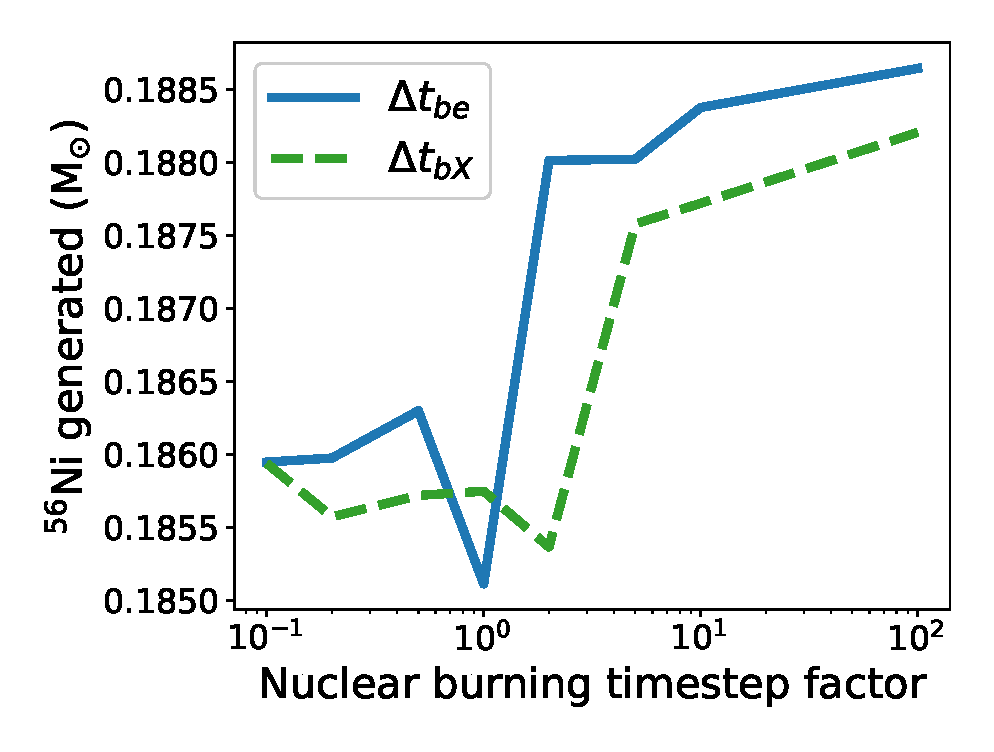
\includegraphics[scale=0.425]{{{plots/dtnuc_max_Ni56_m_P_0.64_m_S_0.64}}}
  \caption{Nickel production as a function of the timestep factors $f_{be}$
           (solid blue, limiting the timestep on changes in internal energy) and
           $f_{bX}$ (dashed green, limiting the timestep on changes in species).
           For a given $f_{be}$, $f_{bX}$ with the same value typically limits
           the timestep by at least an order of magnitude more.
           \label{fig:timestep_factor}}
\end{figure}
\autoref{fig:timestep_factor} demonstrates the effect of both parameters on the nickel
production. As either $f$ becomes small, the restriction on the timestep becomes quite
severe: for $f_{bX} = 0.01$, the minimum timestep in the simulation is smaller than
$2 \times 10^{-9}\ \text{s}$ and the full simulation requires over 750,000 timesteps.
Yet it is clear that even for this steep value of the limiter, which is much stricter
than the limiter used in, e.g., \cite{hawley:2012} and \cite{raskin:2010}, the
simulation has not fully converged in nickel production. These limiters are somewhat
redundant in the sense that a given $f_{bX}$ corresponds to another (higher) $f_{be}$,
as is evident by the fact that on the graph the curves look similar in shape but with
a horizontal offset.

We also examined the effect of the method used to enforce the limiting, using the
four limiting modes discussed in \autoref{sec:hydrocoupling}. The results are shown
in \autoref{table:burninglimitermode} for the case $f_{be} = 0.3$ (we did not use
limiting with $f_{bX}$ for this test). The two modes that use the full last timestep's
worth of information to estimate $\dot{e}$ yield a slightly larger nickel mass than the
two modes that only use more recent information, but the difference is negligible.

\input{plots/burning_limiter_mode_m_P_0.64_m_S_0.64.tbl}

%TODO: add a ``Nonaka plot''

For all remaining tests in this section, unless otherwise stated, we take $f_{be} = 10^2$
and disable limiting with $f_{bX}$ by setting it to a large number. This choice is a balance
between accuracy and efficiency: we avoid the obviously wrong answers that occur for $f_{be} > 10^3$
while ensuring that the timesteps are long enough that the following tests are computationally
inexpensive.



\subsection{Nuclear Network}
\label{sec:parameters:network}

Now we move to a discussion of the effect of including various isotopes
in the nuclear reaction network. In particular we compare the \isoseven, \aproxthirteen,
\aproxnineteen, and \aproxtwentyone\ reaction networks. In all cases we run
the same problem setup, and the unused isotopes (everything but carbon and oxygen)
have their mass fractions in every zone set to a negligibly small number at initialization.
\autoref{table:networks} lists the $^{56}$Ni generation and total energy generation (determined
by subtracting the initial energy from the final energy). The energy generated in the latter
three cases agrees remarkably well, with a less than $0.5\%$ difference. \aproxthirteen\
over-generates nickel at the $2\%$ level compared to the networks with more isotopes, a reasonably
small difference. On the other hand, agreement with \isoseven\ is not very strong, as \isoseven\
generates far too much nickel and far too little energy. Nevertheless while the quantitative
agreement is not there, the collision looks qualitatively similar compared to the evolution with
more complicated networks, so while \isoseven\ should not be used for predicting nucleosynthetic
yields in production science runs, it may still be fair for use in proof-of-concept studies.

\input{plots/networks_m_P_0.64_m_S_0.64.tbl}

\isoseven\ also has the peculiar property that after the detonation had passed through the WDs,
the region at the central contact point did not fully stop burning, yielding a quasistatic energy
release that added a couple of million extra timesteps to the simulation (in addition to the few
hundred it normally takes) before we manually terminated the run. The full effect of these additional
timesteps only amounted to a $10^{-4}$ relative change in the nickel production. By examining the behavior
of zones near the collision point, we discovered the reason for this. The zones in question have a composition that
is approximately $98\%$ Ni and $2\%$ He by mass. For this combination, a direct evaluation of the RHS in
comparison to, say, \aproxthirteen, reveals that $dX/dt$ for these isotopes is off by many orders of magnitude.
This is a consequence of the choice inherent to the network to assume that the isotopes in between $^{28}$Si
and $^{56}$Ni are in an effective equilibrium state. So an advective update that yields even a small change
to the abundances in the zone will very strongly knock the zone out of equilibrium with respect to the burn
step following the advective update. This then causes the burning timestep limiter to kick in and make the
timestep very small so that the advective changes do not cause such strong effects on the burning equilibrium.
This effect is an argument against the use of \isoseven\ for explosive, non-hydrostatic burning problems.



\subsection{Burning Mode}
\label{sec:parameters:burningmode}

In \autoref{sec:burner} we observed that there are several alternatives to the traditional
self-heating approach in a burn. These alternatives are relevant to a collision problem because,
as pointed out by \cite{raskin:2010} and \cite{kushnir:2013}, it is possible for a typical
zone in our simulation to release a very large amount of energy in a burn before it is cooled
off by a subsequent hydrodynamic expansion step, leading to the numerically unstable burning
problem described in \autoref{sec:unstable_burning}. \autoref{table:burningmode} lists nickel
production for the four burning modes described earlier. The hydrostatic burn does produces
slightly more nickel than the self-heating burn, consistent with the idea that by limiting the
energy release from early carbon burning, we can forestall a detonation which is numerically
spurious. Yet the difference is only about 5\%. The reason is that the hydrostatic burn controls
the energy release during the burn, but \textit{not} what happens in the rest of the hydrodynamics
step. And in the hydrodynamics step, the \castro\ algorithm performs multiple EOS calls to ensure
that the temperature is synchronized with the internal energy at various points in the update.
So in practice there is a temperature change due to the burn for our problem. This seems inevitable
for any hydro code unless the hydrodynamics update includes an explicit equation for $T$ that is
independent of what is happening for the internal energy. Similarly, the hybrid burn does not
affect the total nickel production relative to the hydrostatic burn. The hybrid burn only changes
the behavior for zones that have a net negative energy release from the hydrostatic burn, which
occurs only after we have burned to NSE.

\input{plots/burning_mode_m_P_0.64_m_S_0.64.tbl}

In contrast, the suppressed burning mode (modeled after \citet{kushnir:2013}) produces only about
$5 \times 10^{-4}\ \msolar$ of $^{56}$Ni. In a suppressed burn, we ensure that at every evaluation
of the right-hand-side vector for the nuclear network integration, all quantities are scaled by the
same factor, with this factor ensuring that the energy release is not large enough to permit a
spurious detonation. This seems to be equivalent to the method used in \citet{kushnir:2013}. We
reproduce their claim that this suppresses the detonation until later in the collision, after more
material has approached the stalled shock. We also observe that, for a given resolution, the simultaneous
detonations occur slightly outside the initial contact point, near the edges of the stalled shock. They
establish as the main source of error in simulations that produce too little nickel. However, we find
that the resulting detonations are not strong enough to convert a significant amount of material to NSE
conditions; instead, only QSE conditions are reached near the center of the collision, leaving a significant
amount of silicon and sulfur on the domain that is not further processed.



\subsection{Impact Parameter}
\label{sec:parameters:impactparameter}

As the impact parameter varies for a head-on collision, the cross-section of the contact
zone between the two stars varies in size and geometry. In \autoref{fig:impact_parameter}, we
see the dependence of the nickel production on the impact parameter $b$, measured in units
of the WD radius. This test was performed using the 3D setup at our usual base resolution of
400 km. For computational efficiency, timestep limiting based on burning was disabled.
We sampled at $b = 0.0$, $0.01$, $0.02$, $0.03$, $0.04$, $0.05$, and then increasing
in increments of $0.05$. Relative to $b = 0$, there is a slight increase in nickel production for small
but non-zero $b$, which then declines with increasing $b$ except for a bump at $b = 0.5$.
For $b \ge 0.7$, no detonation forms at all, and the merged object remains a stable C/O WD
with $M = 1.2\ \msolar$ at least until $t = 100$.

It is worth nothing that for $b = 0.0$ the nickel production is a bit smaller for the 3D simulation
than its equivalent 2D simulation, the default case described above. There are differences both in
the size of the timestep (which as we saw in \autoref{sec:parameters:timestepping} plays a role in
the total nickel production) and in the discretized nature of the stars; the assumption of perfect
azimuthal symmetry inherent to the 2D simulation breaks down for the 3D simulation, especially at
low resolution, since the zones are rectangular.

\begin{figure}
  \centering
  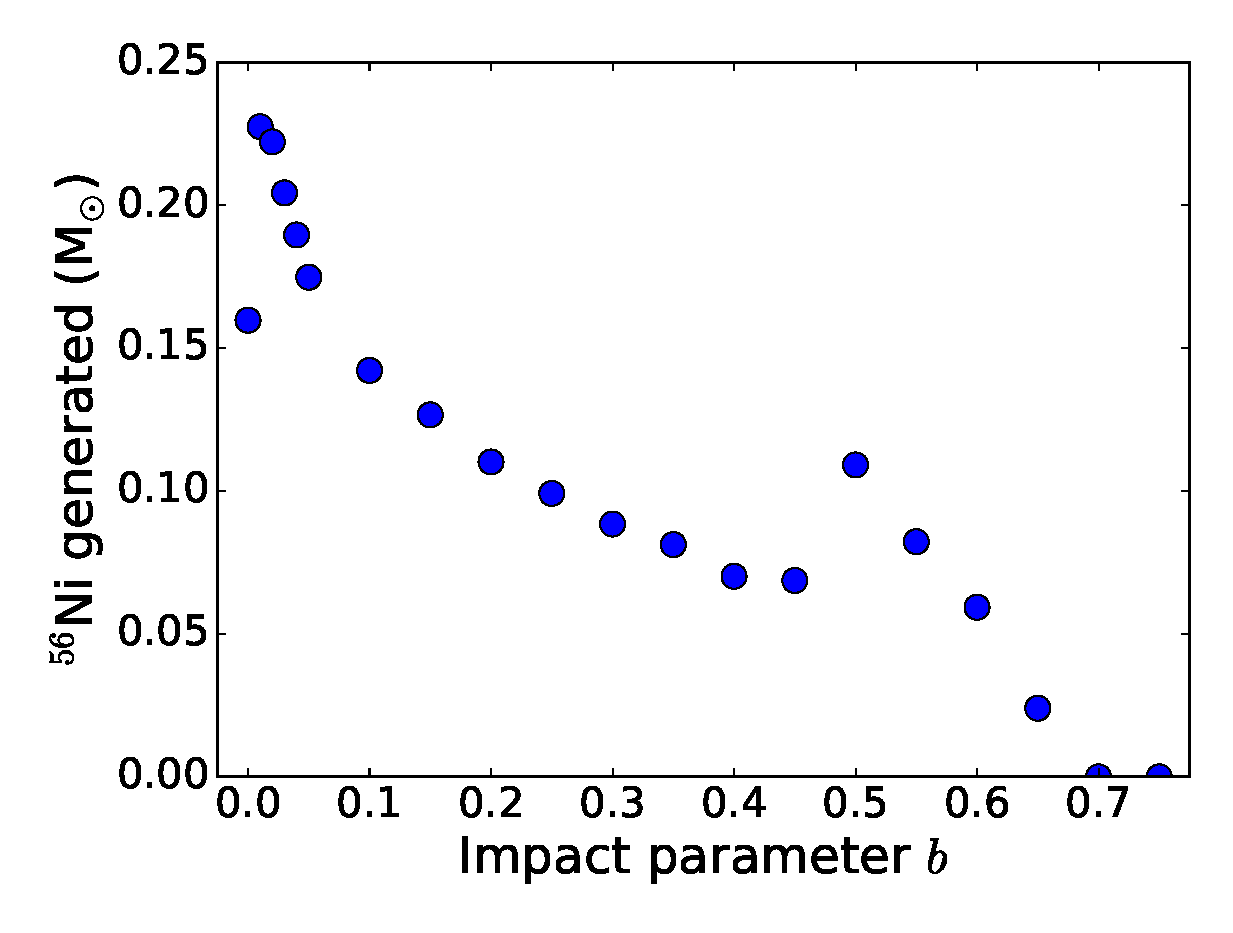
\includegraphics[scale=0.425]{plots/impact_parameter}
  \caption[Nickel production dependence on the impact parameter]
          {$^{56}$Ni generation as a function of the initial WD impact parameter for
           a $0.64\ \msolar$ + $0.64\ \msolar$ WD collision.
           \label{fig:impact_parameter}}
\end{figure}


\subsection{Other Parameters}

We tested a few other parameters that ended up having no serious effect on the outcome.
The dual energy parameter $\eta_2$ described in \autoref{sec:problemsetup} can have a
minor effect on the nickel production, yielding variations on the order of a few percent,
but there is no clear pattern. The dual energy parameter $\eta_3$ has no effect on the
outcome: the answer is the same for $\eta_3 = 0$ and $\eta_3 = 1$, which makes sense
because all of the reacting regions have a low enough kinetic energy relative to their
total energy such that the internal energy variable is always kept in sync with $(E - K)$.
(We did not look at $\eta_1$ because that has a direct effect only on the hydrodynamics,
not the reactions.) We also tested whether our choice for the temperature floor mattered
by lowering it to $10^6\ \text{K}$ and $10^5\ \text{K}$, and this had no effect on nickel
production. It does allow parts of the WDs to become colder as they move, due to numerical
errors in the advecting flow (the Helmholtz equation of state is very insensitive to
temperature, so even small changes in the internal energy can create very large changes
in the implied temperature), but the amount of energy injected by the collision is so
large that the final result is insensitive to whatever the initial temperature of the
WDs were. We also checked whether there was any consequence of our choice to disable the
burning for small enough $\rho$ and $T$. Lowering the minimum $\rho$ for reactions to
$10^0\ \text{g cm}^{-3}$ from $10^6\ \text{g cm}^{-3}$ had a negligible effect,
and varying the minimum $T$ for reactions from $2 \times 10^{7}\ \text{K}$ to
$4 \times 10^{8}\ \text{K}$ also had no meaningful effect.

%TODO: maybe show an image of the temperature field in the WDs before colliding to demonstrate the point about numerical error?

The choice of the WD composition to be equal carbon and oxygen by mass is a common
choice in the literature and is broadly comparable to what stellar evolution codes
yield for WDs of this mass. Still, it is an arbitrary approximation, especially the
insistence that the composition is uniform throughout the WD. In \autoref{table:co}
we list the nickel production as a function of the initial carbon mass fraction.
This can have a few percent impact on the outcome for the plausible values we tested.
In future work we may look at the effect of a more realistic progenitor structure,
including the effects of a helium shell on the surface of the WDs \citep{holcomb:2015}
and a non-uniform interior structure.

\input{plots/co_frac_m_P_0.64_m_S_0.64.tbl}



%==========================================================================
% Resolution Dependence
%==========================================================================
\section{Resolution Dependence}
\label{sec:resolution}



%==========================================================================
% Gravitational Wave Signature
%==========================================================================
\section{Gravitational Wave Signature}
\label{sec:gwsignature}

Paper I established our methodology for calculating the gravitational wave signature
of a white dwarf merger using the post-Newtonian framework of \citet{blanchet:1990}.
While a typical merger event has a characteristic profile including a chirp and ringdown,
white dwarf collisions are noticeably distinct in their gravitational wave signatures, and
hence may be interesting targets for observation for future low frequency gravitational
wave detectors such as LISA \citep{eLISA}. The strain increases monotonically for a collision until impact,
instead of oscillating back and forth at a characteristic frequency as for mergers.
The main caveat for these events compared to events
such as neutron star mergers is that due to the event being inherently less energetic,
the typical distance scale on which we could observe a white dwarf merger or collision
is the size of our own galaxy, with extragalactic events being unlikely to be
detected, at least with the first generation of space-based gravitational wave
detectors.

\begin{figure}
  \centering
  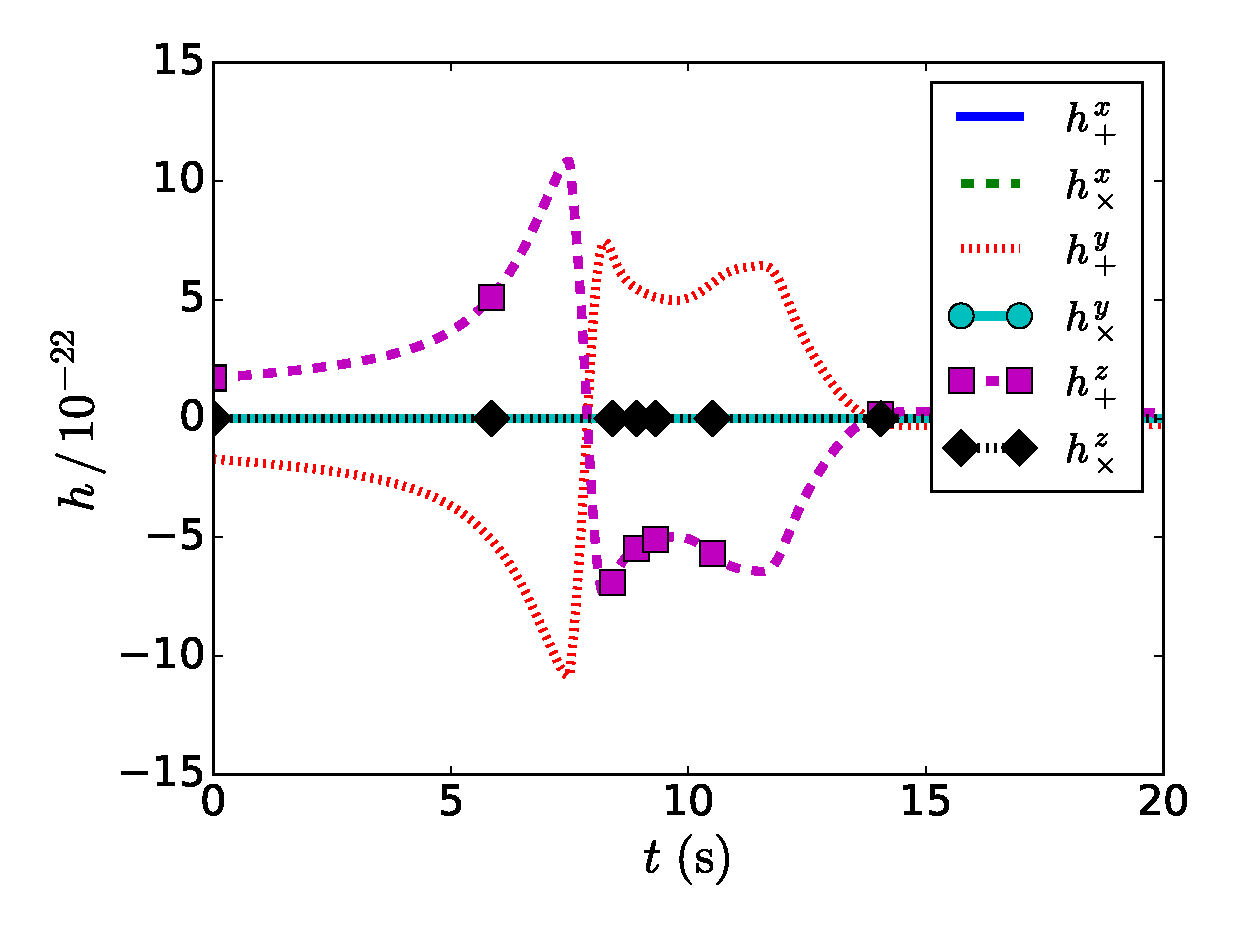
\includegraphics[scale=0.425]{plots/gw_signal_2D}
  \caption{Gravitational wave strains for the head-on collision of two $0.64\ \msolar$
           white dwarfs. The strain is normalized to a source distance of 10 kpc.
           \label{fig:gw_signal_2D}}
\end{figure}

\autoref{fig:gw_signal_2D} is a plot of the gravitational wave strain for
the representative case of \autoref{sec:parameters} ($M_P = 0.64\ \msolar$, $M_S = 0.64\ \msolar$, $b = 0$),
where we disabled the normal stopping criterion and let the simulation run until $t = 20$.
We use the convention that the absolute scale of the strain is normalized to a distance
of 10 kpc (the strain scales inversely with the source distance). We show the $+$ and $\times$
polarizations for observers situated along the $x$, $y$, and $z$ axes (for the 2D case,
this corresponds to the $z$, $R$, and $\phi$ axes, respectively, in the simulation).
The shape of the profile agrees qualitatively with the gravitational wave signatures
predicted by \cite{loren-aguilar:2009:collisions} and \cite{garcia-senz:2013}.
\autoref{fig:gw_signal_3D} shows the strain prediction for a 3D collision event
with $M_P = 0.8\ \msolar$, $M_S = 0.6\ \msolar$, and $b = 0.8$. This mass combination
was chosen because \cite{loren-aguilar:2009:collisions} used the same combination for
gravitational wave signal prediction, but we cannot replicate the large impact parameter
they used on our simulation grid, so the detonation looks quite different than in their case.

\begin{figure}
  \centering
  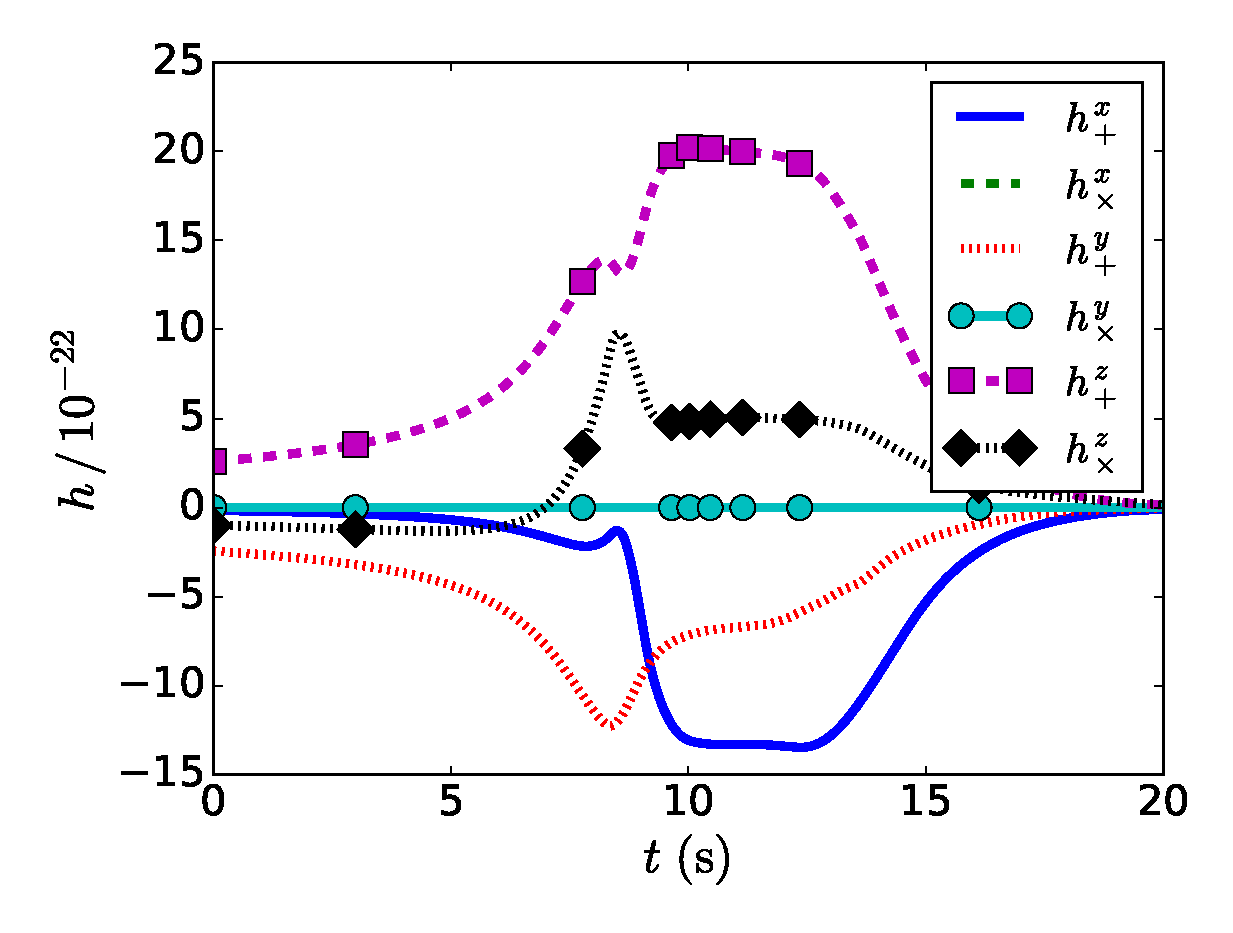
\includegraphics[scale=0.425]{plots/gw_signal_3D}
  \caption{Gravitational wave strains for the off-center collision ($b = 0.8$) of
           $0.8\ \msolar$ and $0.6\ \msolar$ WDs. The strain is normalized to a
           source distance of 10 kpc.
           \label{fig:gw_signal_3D}}
\end{figure}



%==========================================================================
% Conclusions
%==========================================================================
\section{Conclusions and Discussion}\label{Sec:Conclusions and Discussion}
\label{sec:conclusion}



\acknowledgments

This research was supported by NSF award AST-1211563 and DOE/Office of
Nuclear Physics grant DE-FG02-87ER40317 to Stony Brook. An award of
computer time was provided by the Innovative and Novel Computational
Impact on Theory and Experiment (INCITE) program.  This research used
resources of the Oak Ridge Leadership Computing Facility located in
the Oak Ridge National Laboratory, which is supported by the Office of
Science of the Department of Energy under Contract
DE-AC05-00OR22725. Project AST106 supported use of the ORNL/Titan
resource.  This research used resources of the National Energy
Research Scientific Computing Center, which is supported by the Office
of Science of the U.S. Department of Energy under Contract
No. DE-AC02-05CH11231.  Results in this paper were obtained using the
high-performance LIred computing system at the Institute for Advanced
Computational Science at Stony Brook University, which was obtained
through the Empire State Development grant NYS \#28451.

This research has made use of NASA's Astrophysics Data System 
Bibliographic Services. In addition, this research has made use
of the AstroBetter blog and wiki.

\software{BoxLib\footnote{\url{https://github.com/BoxLib-Codes/BoxLib}},
          CASTRO \citep{castro} (https://github.com/BoxLib-Codes/Castro),
          wdmerger \citep{wdmergerI} (\url{https://github.com/BoxLib-Codes/wdmerger}),
          GCC (\url{https://gcc.gnu.org/}),
          python (\url{https://www.python.org/}),
          matplotlib \citep{matplotlib}, \url{http://matplotlib.org/}),
          yt \citep{yt}, \url{http://yt-project.org/})}

\clearpage

\bibliographystyle{../aasjournal}
\bibliography{../refs}

\end{document}
